\section{Les BUS de la GTB}
Pour mettre en oeuvre une GTB, l'automate doit pouvoir communiquer avec les différents équipements du bâtiment (capteurs, actionneurs, superviseur, etc.). Cette communication est réalisée par l'intermédiaire de BUS de terrain. Certains de ces BUS sont normalisés, d'autres sont propriétaires.\\

\begin{UPSTIactivite}[][Architecture détaillée d'une GTB]
	\UPSTIeleveOnly{\vspace{9cm}}
	\UPSTIprofOnly{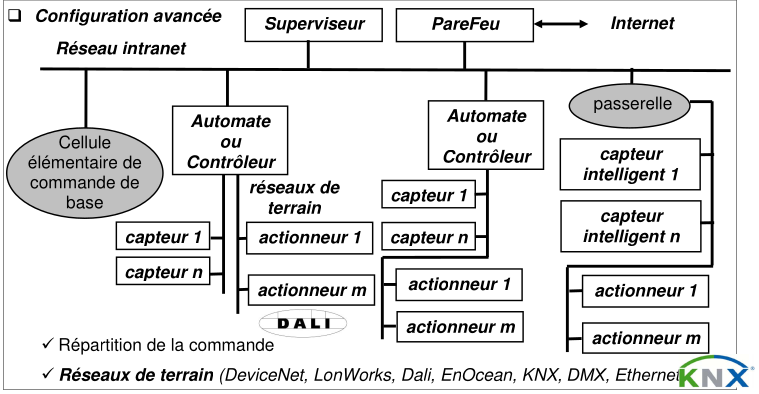
\includegraphics[height=8.5cm]{architectureDetailleeGTB}}
\end{UPSTIactivite}

Exemple de protocoles de réseaux de terrain : 
\begin{multicols}{4}
	\begin{itemize}
		\item KNX,
		\item Modbus,
		\item BACnet.
		\item LonWorks.
		\item M-Bus.
		\item DALI.
		\item EnOcean.
		\item ZigBee.
	\end{itemize}
\end{multicols}

\pagebreak
\subsection{Le bus DALI}

	Le bus DALI (Digital Adressable Lighting Interface) est un bus de communication normalisé permettant de piloter individuellement des luminaires. Créé en 1999 par un consortium de fabricants de luminaires, il est normalisé par la norme IEC 62386. DALI2 a ensuite été introduit en 2014 pour quelques améliorations et, plus récemment, DALI+. 
	
	Il s'agit d'un bus maître/esclave. L'automate joue le rôle du maître et envoie des ordres aux esclaves (les luminaires). Ces derniers répondent en envoyant des trames de retour.\\
	\begin{multicols}{2}
			\begin{description}
		\item[Tension] 16 V
		\item[Courant] 250 mA
		\item[Longueur maximale] 300 m
		\item[Débit] 1200 bauds
		\item[Codage] Manchester
		\item[Câblage] Paire différentielle torsadée
	\end{description}
	\end{multicols}


	\begin{UPSTIactivite}[][Structure d'un réseau DALI]
		\UPSTIeleveOnly{\vspace{6cm}}
		\UPSTIprofOnly{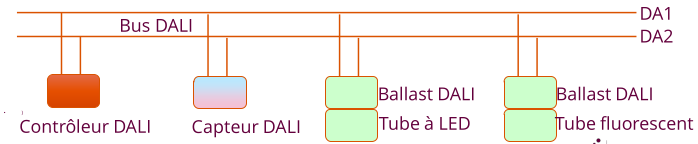
\includegraphics[height=3cm]{architectureDALI}\\\vspace{2.5cm}}
	\end{UPSTIactivite}

	Une trame DALI est composée de 19 bits : 1 bit de start, 8 bits d'adresse, 8 bits de données et 2 bits de stop.\\ La trame de réponse est composée de 11 bits : 1 bit de start, 8 bits de données et 2 bits de stop.\\

	Chaque actionneur est identifié par une adresse codée sur 6 bits. La structure de l'octet d'adresse pour s'adresser à un actionneur spécifique est alors la suivante : 
	\begin{center}
		\begin{tabular}{|c|c|c|c|c|c|c|c|}
			\hline
			B7 & B6 & B5 & B4 & B3 & B2 & B1 & B0\\
			\hline
			0 & A5 & A4 & A3 & A2 & A1 & A0 & S\\
			\hline
		\end{tabular}
	\end{center}

	Il est également possible de regrouper plusieurs actionneurs sous une même adresse. On peut mémoriser 16 adresses de groupes, codées sur 4 bits. La structure de l'octet d'adresse pour s'adresser à un groupe d'actionneurs est alors la suivante :
	
	\begin{center}
		\begin{tabular}{|c|c|c|c|c|c|c|c|}
			\hline
			B7 & B6 & B5 & B4 & B3 & B2 & B1 & B0\\
			\hline
			1 & 0 & 0 & A3 & A2 & A1 & A0 & S\\
			\hline
		\end{tabular}
	\end{center}

	Le bit \textit{S} sert à indiquer le type de commande que l'on enverra ensuite. Si \textit{S} vaut 0, on enverra une valeur contrôlant directement la luminosité du luminaire. Si \textit{S} vaut 1, on enverra une commande spéciale (voir tableau des commandes en annexe).\\

	Le contrôle de la luminosité du luminaire se fait sur 8 bits. La valeur 0 correspond à une luminosité de 0\% et la valeur 255 correspond à une luminosité de 100\%. La formule de conversion est $P = \frac{P_{\text{nom}}}{10}\times10^{\frac{x-1}{253/3}}$ dont la courbe est donnée ci-dessous : 

	 \begin{center}
		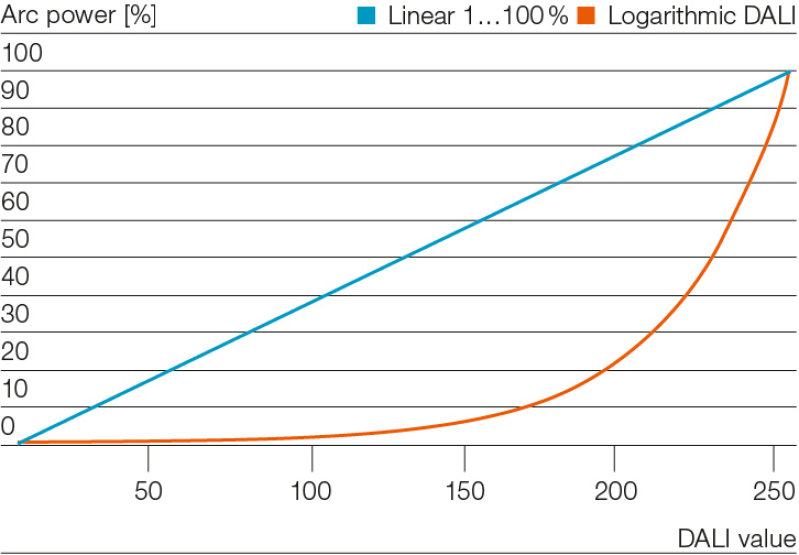
\includegraphics[width=.7\textwidth]{courbeDALI}
	% 	\begin{pdfdisplay}
	% 	\begin{pspicture}(-2.5,-1)(2.5,5)
	% 		\psset{xunit=1 cm, algebraic=true}
	% 		\psaxes{->}(0,0)(-2.5,-1)(2.5,5)
	% 		\psplot[linewidth=1.5pt]{-2}{2}{x^2}
	% 		\end{pspicture}
	% 		\end{pdfdisplay}
	\end{center}

	\begin{UPSTIactivite}[][Exemple de trame DALI]
		\UPSTIquestion Donner la trame à envoyer pour allumer le luminaire d'adresse 54 à 50\% de sa puissance.
		\vspace{1cm}
		\UPSTIquestion Donner la trame à envoyer pour augmenter la luminosité du luminaire d'adresse 54 de 1.  
		\vspace{1cm}
	\end{UPSTIactivite}

	\subsection{Distribution de l'énergie}
	\begin{figure}[h!]
		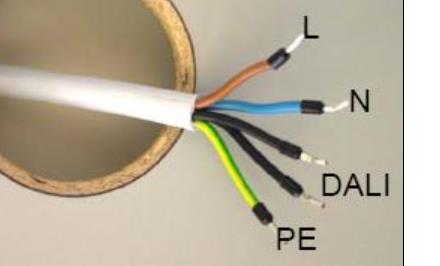
\includegraphics[height=.15\textheight]{cableDALI}
		\hfill
		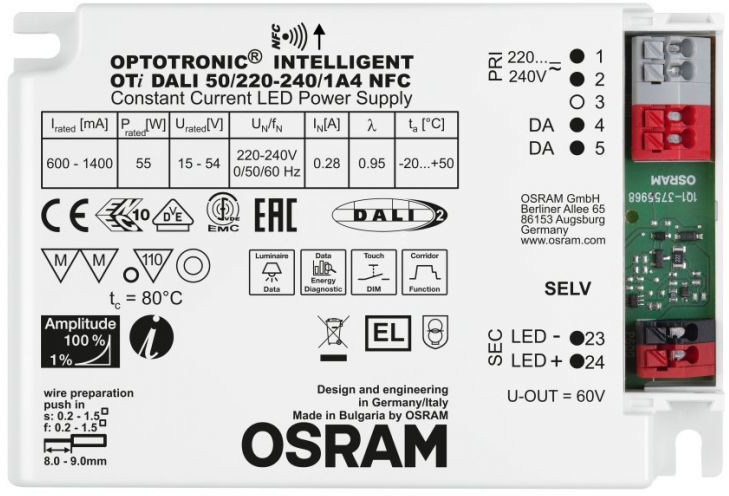
\includegraphics[height=.15\textheight]{ballastDALI}
		\caption{Cable et ballast DALI}
	\end{figure}

	Un câble DALI transporte habituellement, en plus des données, l'énergie alimentant les actionneurs. Il est donc composé de 5 fils : 3 fils pour l'alimentation (Neutre, Phase et Terre) et 2 fils pour la communication (A et B).\\

	\begin{UPSTIactivite}[][Architecture DALI]
		\UPSTIeleveOnly{\vspace{8cm}}
		\UPSTIprofOnly{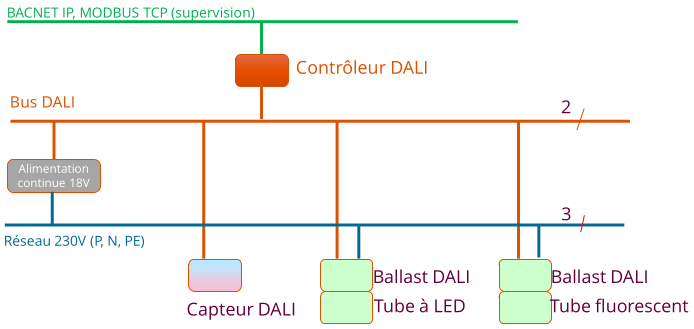
\includegraphics[height=7.5cm]{energieDALI}}
	\end{UPSTIactivite}





